\subsection{Demand Calculation} \label{demandCalc}

%\gls{sCP}  % sumComponentPrices
%\gls{dPR}  % demandPrice
%\gls{sP}  % salesPrice
%\gls{tD}  % totalDemand
%\gls{nOP}  % numberOfferedProducts
%\gls{mS}  % marketShare
%\gls{tMS}  % totalMarketShare
%\gls{sFP}  % salesFigureProduct
%\gls{dPC}  % demandPercentage
%\gls{tP}  % totalPopulation

In Capitalism X, we assume that the demand for a product is based on customer satisfaction and the selling price. In addition, there is the assumption that the population is aware of the prices of the latest individual components. So they can estimate the value of the product from its components only, if the company uses the latest ones.
 
Table \ref{sum_product_component_prices} shows the sum of the component prices (\gls{sCP}), the current components and their respective prices were used for the calculation.

\begin{table}[ht]
    \centering
    \begin{tabular}{|l|r|r|r|r|r|r|r|r|r|r|}
    \hline
                & \textbf{1990} & \textbf{1991}  & \textbf{1992}  & \textbf{1993}  & \textbf{1994}  & \textbf{1995}  & \textbf{1996}  & \textbf{1997}  & \textbf{1998}  & \textbf{1999}  \\
    \textbf{Notebook}    & 1380  & 1383  & 1354  & 1330  & 1309  & 1665  & 1661  & 1505  & 1493  & 1477  \\   
    \textbf{Phone}       & 610   & 612   & 589   & 575   & 562   & 518   & 516   & 458   & 452   & 441   \\ 
    \textbf{Game Boy}    & 27    & 29    & 17    & 12    & 12    & 12    & 22    & 23    & 17    & 36    \\  
    \textbf{Television}  & 370   & 372   & 349   & 335   & 322   & 296   & 292   & 270   & 256   & 244    \\ 
    \hline       
                & \textbf{2000}  & \textbf{2001}  & \textbf{2002}  & \textbf{2003}  & \textbf{2004}  & \textbf{2005}  & \textbf{2006}  & \textbf{2007}  & \textbf{2008}  & \textbf{2009} \\
    \textbf{Notebook}    & 1283  & 1356  & 1529  & 1462  & 1400  & 1425  & 1378  & 1365  & 1057  & 1136 \\   
    \textbf{Phone}       & 427   & 421   & 405   & 390   & 443   & 439   & 424   & 437   & 439   & 410 \\  
    \textbf{Game Boy}    & 37    & 26    & 16    & 24    & 54    & 50    & 44    & 40    & 54    & 51  \\   
    \textbf{Television}  & 318   & 316   & 297   & 286   & 277   & 450   & 452   & 435   & 422   & 415 \\ 
    \hline
                & \textbf{2010}  & \textbf{2011}  & \textbf{2012}  & \textbf{2013}  & \textbf{2014}  & \textbf{2015}  & \textbf{2016}  & \textbf{2017}  &  &\\
    \textbf{Notebook}    & 1233  & 1220  & 1364  & 1492  & 1480  & 1416  & 1411  & 1395  &  &\\   
    \textbf{Phone}       & 386   & 365   & 352   & 312   & 311   & 342   & 333   & 333   &  &\\ 
    \textbf{Game Boy}    & 37    & 59    & 61    & 53    & 44    & 48    & 40    & 26    & & \\  
    \textbf{Television}  & 334   & 344   & 329   & 322   & 316   & 233   & 237   & 228   &  &\\ 
    \hline
    \end{tabular}
    \caption{Sum product component prices}
    \label{sum_product_component_prices}
\end{table}
 
The customer satisfaction influences the interest of the population in the respective products by shifting the price at which 100\% are interested. In the following this price is called demand Price (\gls{dPR}).
 
The more satisfied customers are with the company, the more they are willing to pay for the same products. However, if customer satisfaction falls below 40, the demand price falls below the assumed component cost that the company has. The following formula shows how customer satisfaction affects the price at which 100\% of the population demand a product.
\begin{equation}
\label{func:demandPrice}
\begin{aligned}
if ( cS \geq 80 ) { dPR = sCP * 1,2 } \\
elseif ( 80 > cS \geq 60 ){ dPR = sCP * 1,1 } \\
elseif ( 60 > cS \geq 50 ) { dPR = sCP * 1,05 } \\
elseif ( 50 > cS \geq 40 ) { dPR = sCP * 1 } \\
elseif ( 40 > cS \geq 20 ) { dPR = sCP * 0,9 } \\
else { dPR = sCP * 0,8 }  
\end{aligned}
\end{equation}

The demand in percentage (\gls{dPC}) is calculated by determining the ratio of the sales price (\gls{sP}) of the product to its demand price and using it as input for the following formula.
\begin{equation}
\label{func:demandPercentage}
\begin{aligned}
x = sP / dPR \\
dPC = 167.905104 * e^{−2.990914872 * 10^{ -1* } x^{ 2 } } \\
if the result is > 100; dPC = 100\% \\
if the result is < 0; dPC = 0\% \\    
\end{aligned}
\end{equation}

chart \ref{jpg:demandFunction} shows the course of the demand function for the demand price of 1,000 CapCoins. 

\begin{figure}
	\centering
	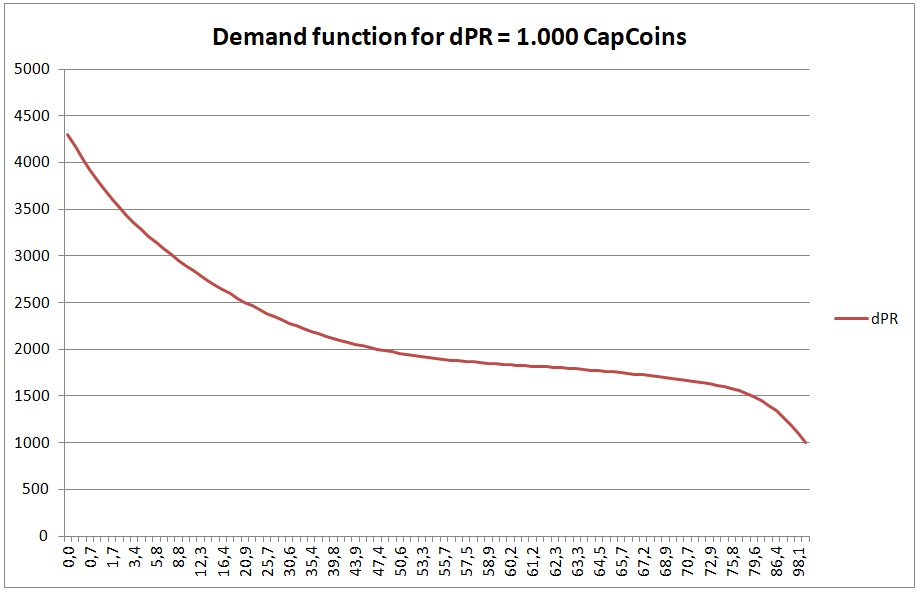
\includegraphics[width=12cm]{images/demandFunction.jpg}
	\caption{Demand function or dPR = 1.000 CapCoins}
	\label{jpg:demandFunction}
\end{figure}
 
The absolute demand (\gls{tD}) for a product is finally calculated by combining the demand in percent with the population number (\gls{tP}). This approach enables the total demand to be higher than the actual quantity of products offered.
\begin{equation}
tD= dPC * tP    
\end{equation}

The quantity actually sold by the company, so-called sales figures per product (\gls{sFP}), depends on whether the actual demand exceeds the quantity of products offered (\gls{nOP}) or not.
\begin{equation}
\label{func:salesFigure}
\begin{aligned}
if ( tD > nOP ) { sFP = nOP } \\
else { sFP = tD }    
\end{aligned}
\end{equation}

For the calculation of the market share (\gls{mS}) it is assumed that the proportion of the population who would have liked to buy a product but went away empty-handed buys its product from a competitor. The company's total market share (\gls{tMS}) is calculated using the sum of the sales figures of the single products and the sum of the demands for them. Following formulas show the calculation of the market share of a product and the total market share of the company.  
\begin{equation}
\label{func:marketShare}
mS = sFP / tD
tMS = sum(sFP) / sum(tD)   
\end{equation}

